\tikzset{>=latex} % for LaTeX arrow head
\colorlet{xcol}{blue!70!black}
\tikzstyle{rvec}=[->,thick,xcol,line cap=round]

% VECTOR breakdown on axis
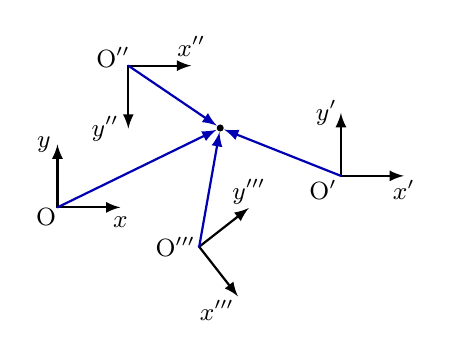
\begin{tikzpicture}
  \small
  \def\L{0.8}
  \def\R{2.3}
  \def\ang{26}
  \def\thet{-52}
  \coordinate (O) at (0,0);
  \coordinate (O1) at (3.6,0.4);
  \coordinate (O2) at (0.9,1.8);
  \coordinate (O3) at (1.8,-0.5);
  \coordinate (R) at (\ang:\R);
  \node[fill=black,circle,inner sep=0.9] (R') at (R) {};
  
  % O1
  \draw[<->,thick] (\L,0) node[below] {$x$} --
                   (O) node[below left=-3] {O} --
                   (0,\L) node[left=-1] {$y$};
  \draw[rvec] (O) -- (R');
  
  % O1
  \begin{scope}[shift={(O1)}]
    \draw[<->,thick] (\L,0) node[below=-2] {$x'$} --
                     (0,0) node[below left=-2] {O$'$} --
                     (0,\L) node[left=-2] {$y'$};
    \draw[rvec] (0,0) -- (R');
  \end{scope}
  
  % O2
  \begin{scope}[shift={(O2)}]
    \draw[<->,thick] (\L,0) node[above] {$x''$} --
                     (0,0) node[above left=-4] {O$''$} --
                     (0,-\L) node[left] {$y''$};
    \draw[rvec] (0,0) -- (R');
  \end{scope}
  
  % O3
  \begin{scope}[shift={(O3)}]
    \draw[<->,thick] (\thet:\L) node[below left=-2] {$x'''$} --
                     (0,0) node[left=-2] {O$'''$} --
                     (\thet+90:\L) node[above=-2] {$y'''$};
    \draw[rvec] (0,0) -- (R');
  \end{scope}
  
\end{tikzpicture}